\documentclass[13pt,onlymath]{beamer}
\usefonttheme{serif}
\usepackage{graphicx,amsmath,amssymb,tikz,psfrag,epstopdf,fancyvrb}
\usepackage[lighttt]{lmodern}
%\usepackage{graphicx,psfrag}

\input defs.tex

%% formatting

\mode<presentation>
{
\usetheme{default}
}
\setbeamertemplate{navigation symbols}{}
\usecolortheme[rgb={0.13,0.28,0.59}]{structure}
\setbeamertemplate{itemize subitem}{--}
\setbeamertemplate{frametitle} {
    \begin{center}
      {\large\bf \insertframetitle}
    \end{center}
}

\newcommand\footlineon{
  \setbeamertemplate{footline} {
    \begin{beamercolorbox}[ht=2.5ex,dp=1.125ex,leftskip=.8cm,rightskip=.6cm]{structure}
      \footnotesize \insertsection
      \hfill
      {\insertframenumber}
    \end{beamercolorbox}
    \vskip 0.45cm
  }
}
\footlineon

\AtBeginSection[] 
{ 
    \begin{frame}<beamer> 
        \frametitle{Outline} 
        \tableofcontents[currentsection,currentsubsection] 
    \end{frame} 
} 

%% begin presentation

\title{\large \bfseries Network Flow Problems}

\author{Jaehyun Park\\[3ex]
CS 97SI\\
Stanford University}

\date{\today}

\begin{document}

\frame{
\thispagestyle{empty}
\titlepage
}

\section{Network Flow Problems}

\begin{frame}{Network Flow Problem}
\BIT
\item A type of network optimization problem
\item Arise in many different contexts (CS 261):
\BIT
\item Networks: routing as many packets as possible on a given network
\item Transportation: sending as many trucks as possible, where roads have limits on the number of trucks per unit time
\item Bridges: destroying (?!) some bridges to disconnect $s$ from $t$, while minimizing the cost of destroying the bridges
\EIT \EIT
\end{frame}

\begin{frame}{Network Flow Problem}
\BIT
\item Settings: Given a directed graph $G = (V, E)$, where each edge $e$ is associated with its capacity $c(e) > 0$. Two special nodes source $s$ and sink $t$ are given $(s \ne t)$
\vfill
\item Problem: Maximize the total amount of flow from $s$ to $t$ subject to two constraints
\BIT
\item Flow on edge $e$ doesn't exceed $c(e)$
\item For every node $v\ne s, t$, incoming flow is equal to outgoing flow
\EIT \EIT
\end{frame}

\begin{frame}{Network Flow Example (from CLRS)}
\BIT
\item Capacities
\begin{center}
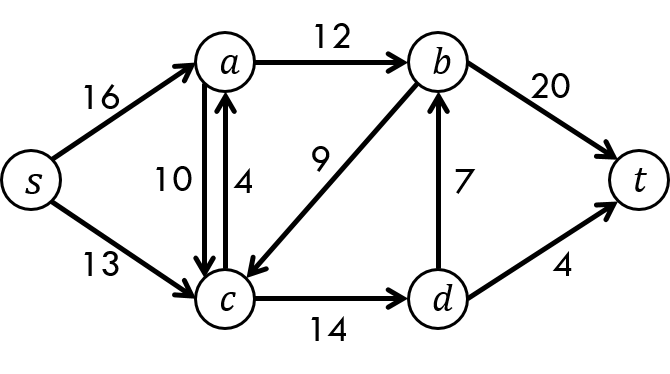
\includegraphics[height=0.3\textheight]{figures/flow_example1}
\end{center}
\vfill
\item Maximum flow (of 23 total units)
\begin{center}
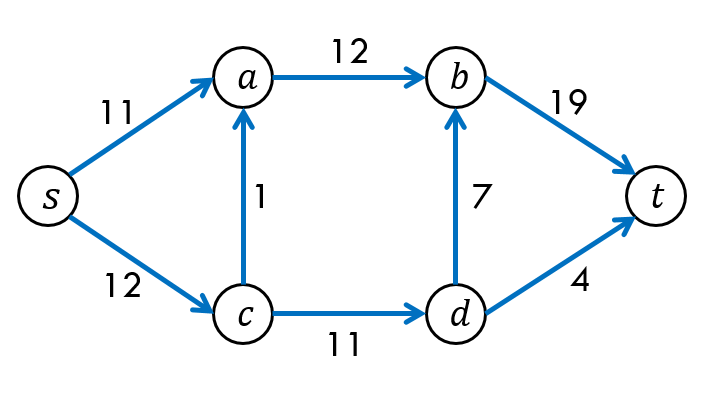
\includegraphics[height=0.3\textheight]{figures/flow_example2}
\end{center}
\EIT
\end{frame}

\begin{frame}{Alternate Formulation: Minimum Cut}
\BIT
\item We want to remove some edges from the graph such that after removing the edges, there is no path from $s$ to $t$
\item The cost of removing $e$ is equal to its capacity $c(e)$
\item The minimum cut problem is to find a cut with minimum total cost
\vfill
\item Theorem: $(\mbox{maximum flow}) = (\mbox{minimum cut})$
\item Take CS 261 if you want to see the proof
\EIT
\end{frame}

\begin{frame}{Minimum Cut Example}
\BIT
\item Capacities
\begin{center}
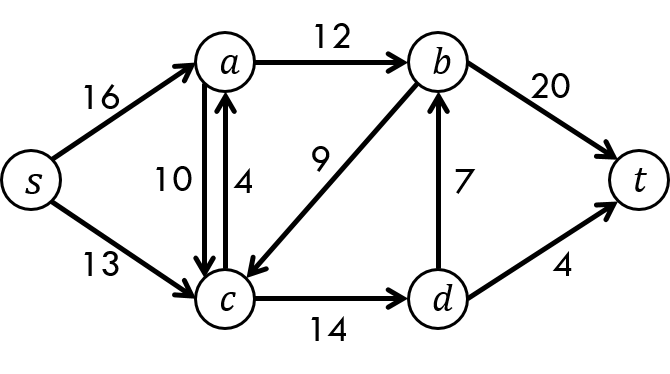
\includegraphics[height=0.3\textheight]{figures/flow_example1}
\end{center}
\vfill
\item Minimum Cut (red edges are removed)
\begin{center}
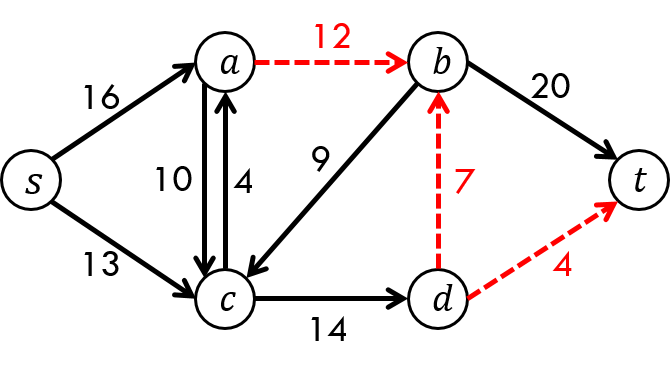
\includegraphics[height=0.3\textheight]{figures/mincut_example}
\end{center}
\EIT
\end{frame}

\begin{frame}{Flow Decomposition}
\BIT
\item Any valid flow can be decomposed into flow paths and circulations
\begin{center}
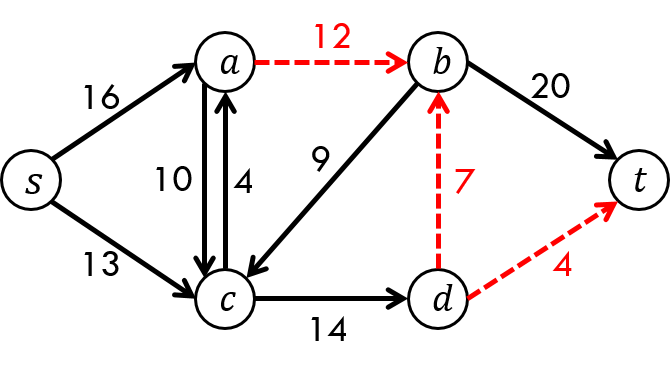
\includegraphics[height=0.3\textheight]{figures/mincut_example}
\end{center}
\BIT
\item $s \rightarrow a \rightarrow b \rightarrow t$: 11
\item $s \rightarrow c \rightarrow a \rightarrow b \rightarrow t$: 1
\item $s \rightarrow c \rightarrow d \rightarrow b \rightarrow t$: 7
\item $s \rightarrow c \rightarrow d \rightarrow t$: 4
\EIT \EIT
\end{frame}

\section{Ford-Fulkerson Algorithm}

\begin{frame}{Ford-Fulkerson Algorithm}
\BIT
\item A simple and practical max-flow algorithm
\item Main idea: find valid flow paths until there is none left, and add them up
\item How do we know if this gives a maximum flow?
\BIT
\item Proof sketch: Suppose not. Take a maximum flow $f^\star$ and ``subtract'' our flow $f$. It is a valid flow of positive total flow. By the flow decomposition, it can be decomposed into flow paths and circulations. These flow paths must have been found by Ford-Fulkerson. Contradiction.
\EIT \EIT
\end{frame}

\begin{frame}{Back Edges}
\BIT
\item We don't need to maintain the amount of flow on each edge but work with capacity values directly
\item If $f$ amount of flow goes through $u\rightarrow v$, then:
\BIT
\item Decrease $c(u\rightarrow v)$ by $f$
\item Increase $c(v\rightarrow u)$ by $f$
\EIT
\item Why do we need to do this?
\BIT
\item Sending flow to both directions is equivalent to canceling flow
\EIT \EIT
\end{frame}

\begin{frame}{Ford-Fulkerson Pseudocode}
\BIT
\item Set $f_\mathrm{total} = 0$
\item Repeat until there is no path from $s$ to $t$:
\BIT
\item Run DFS from $s$ to find a flow path to $t$
\item Let $f$ be the minimum capacity value on the path
\item Add $f$ to $f_\mathrm{total}$
\item For each edge $u \rightarrow v$ on the path:
\BIT
\item Decrease $c(u\rightarrow v)$ by $f$
\item Increase $c(v\rightarrow u)$ by $f$
\EIT \EIT \EIT
\end{frame}

\begin{frame}{Analysis}
\BIT
\item Assumption: capacities are integer-valued
\item Finding a flow path takes $\Theta(n+m)$ time
\item We send at least 1 unit of flow through the path
\item If the max-flow is $f^\star$, the time complexity is $O((n+m)f^\star)$
\BIT
\item ``Bad'' in that it depends on the output of the algorithm
\item Nonetheless, easy to code and works well in practice
\EIT \EIT
\end{frame}

\begin{frame}{Computing Min-Cut}
\BIT
\item We know that max-flow is equal to min-cut
\item And we now know how to find the max-flow
\vfill
\item Question: how do we find the min-cut?
\item Answer: use the residual graph
\EIT
\end{frame}

\begin{frame}{Computing Min-Cut}
\BIT
\item ``Subtract'' the max-flow from the original graph
\EIT
\begin{center}
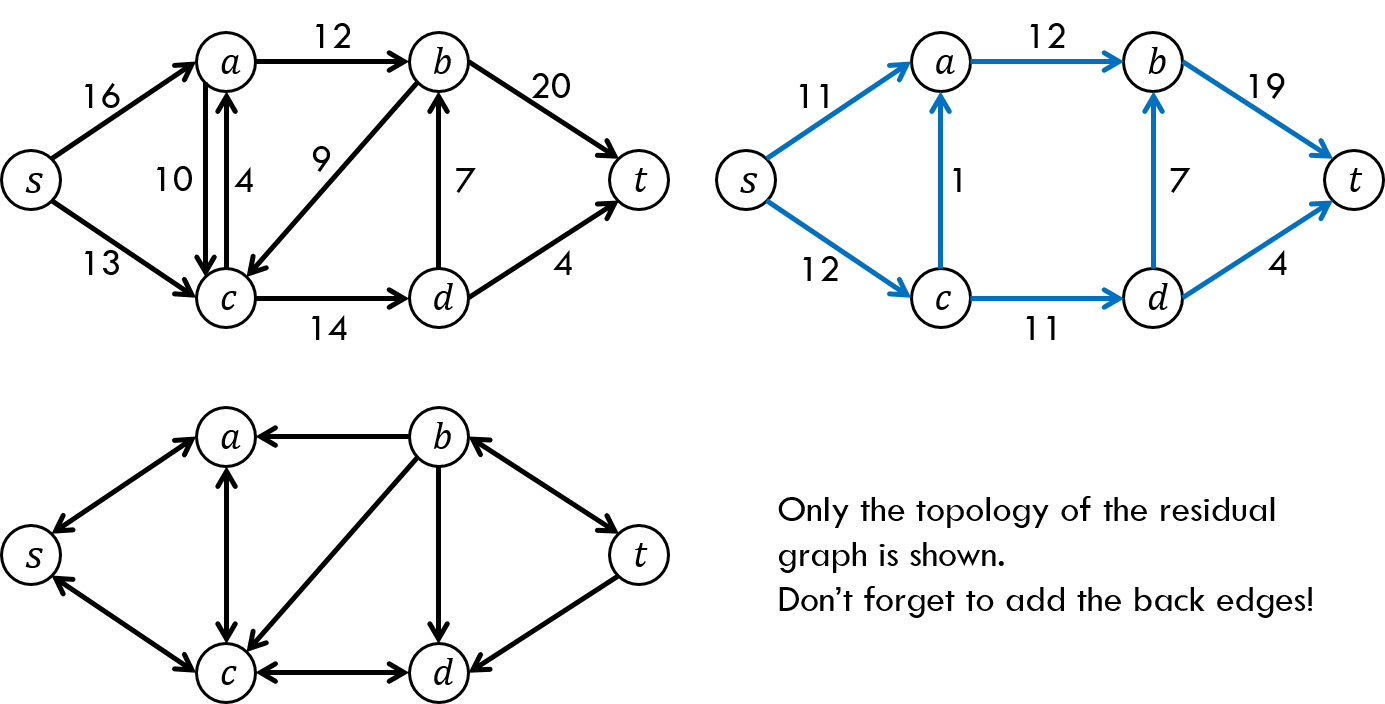
\includegraphics[height=0.6\textheight]{figures/mincut_computation1}
\end{center}
\end{frame}

\begin{frame}{Computing Min-Cut}
\BIT
\item Mark all nodes reachable from $s$
\BIT
\item Call the set of reachable nodes $A$
\EIT
\begin{center}
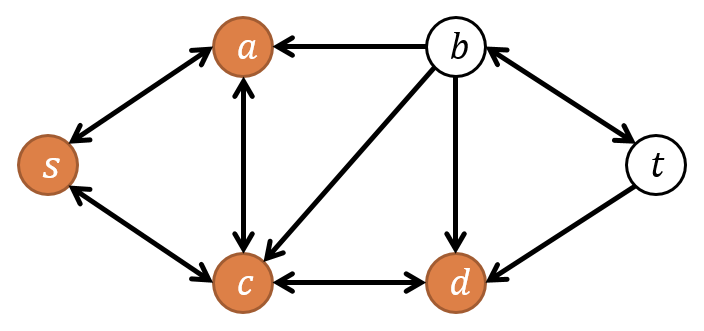
\includegraphics[height=0.3\textheight]{figures/mincut_computation2}
\end{center}
\vfill
\item Now separate these nodes from the others
\BIT
\item Cut edges going from $A$ to $V-A$
\EIT \EIT
\end{frame}

\begin{frame}{Computing Min-Cut}
\BIT
\item Look at the original graph and find the cut:
\begin{center}
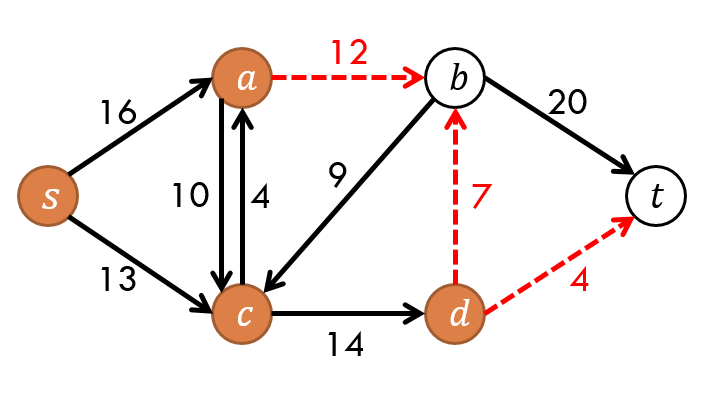
\includegraphics[height=0.35\textheight]{figures/mincut_computation3}
\end{center}
\vfill
\item Why isn't $b\rightarrow c$ cut?
\EIT
\end{frame}

\section{Bipartite Matching}

\begin{frame}{Bipartite Matching}
\BIT
\item Settings:
\BIT
\item $n$ students and $d$ dorms
\item Each student wants to live in one of the dorms of his choice
\item Each dorm can accommodate at most one student (?!)
\BIT
\item Fine, we will fix this later...
\EIT \EIT
\vfill
\item Problem: find an assignment that maximizes the number of students who get a housing
\EIT
\end{frame}

\begin{frame}{Flow Network Construction}
\BIT
\item Add source and sink
\item Make edges between students and dorms
\BIT
\item All the edge weights are 1
\EIT \EIT
\begin{center}
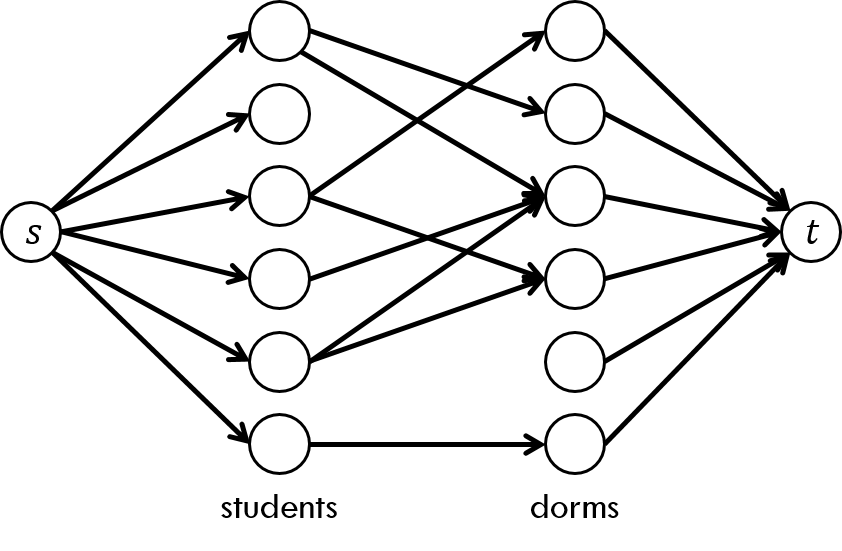
\includegraphics[height=0.5\textheight]{figures/bimatching_construction1}
\end{center}
\end{frame}

\begin{frame}{Flow Network Construction}
\BIT
\item Find the max-flow
\item Find the optimal assignment from the chosen edges
\EIT
\begin{center}
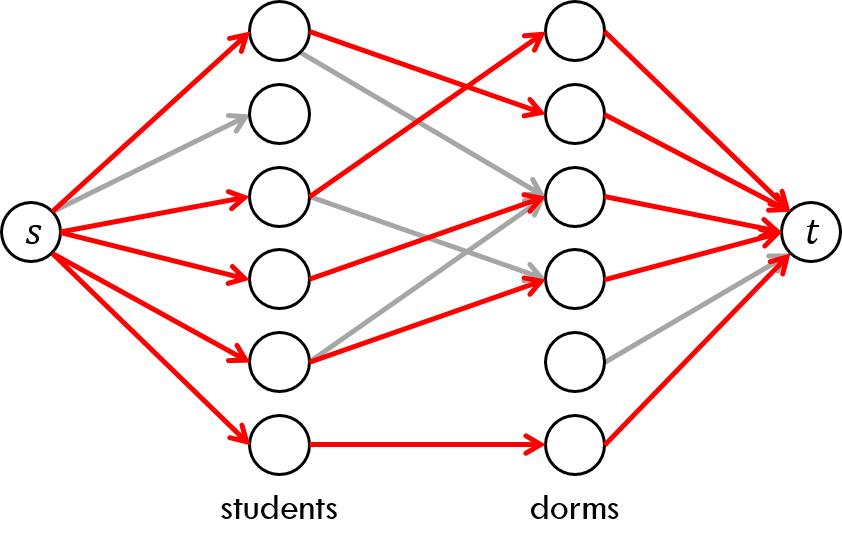
\includegraphics[height=0.5\textheight]{figures/bimatching_construction2}
\end{center}
\end{frame}

\begin{frame}{Related Problems}
\BIT
\item A more reasonable variant of the previous problem: dorm $j$ can accommodate $c_j$ students
\BIT
\item Make an edge with capacity $c_j$ from dorm $j$ to the sink
\EIT
\item Decomposing a DAG into nonintersecting paths
\BIT
\item Split each vertex $v$ into $v_\mathrm{left}$ and $v_\mathrm{right}$
\item For each edge $u\rightarrow v$ in the DAG, make an edge from $u_\mathrm{left}$ to $v_\mathrm{right}$
\EIT
\item And many others...
\EIT
\end{frame}


\section{Min-cost Max-flow Algorithm}

\begin{frame}{Min-Cost Max-Flow}
\BIT
\item A variant of the max-flow problem
\item Each edge $e$ has capacity $c(e)$ and cost $\mathrm{cost}(e)$
\item You have to pay $\mathrm{cost}(e)$ amount of money per unit flow flowing through $e$
\item Problem: find the maximum flow that has the minimum total cost
\item A lot harder than the regular max-flow
\BIT
\item But there is an easy algorithm that works for small graphs
\EIT\EIT
\end{frame}

\begin{frame}{Simple (?) Min-Cost Max-Flow}
\BIT
\item Forget about the costs and just find a max-flow
\item Repeat:
\BIT
\item Take the residual graph
\item Find a negative-cost cycle using Bellman-Ford
\BIT
\item If there is none, finish
\EIT
\item Circulate flow through the cycle to decrease the total cost, until one of the edges is saturated
\BIT
\item The total amount of flow doesn't change!
\EIT\EIT
\item Time complexity: very slow
\EIT
\end{frame}

\begin{frame}{Notes on Max-Flow Problems}
\BIT
\item Remember different formulations of the max-flow problem
\BIT
\item Again, $(\mbox{maximum flow})=(\mbox{minimum cut})$!
\EIT
\item Often the crucial part is to construct the flow network
\item We didn't cover fast max-flow algorithms
\BIT
\item Refer to the Stanford Team notebook for efficient flow algorithms
\EIT \EIT
\end{frame}

\end{document}
